\documentclass{beamer}
\usepackage{HECbeamer}
\usepackage{icomma}
\usepackage{numprint}
\title[\color{white}{MATH 60604 \S~5h - Hétéroscédasticité de groupe}]{\texorpdfstring{MATH 60604 \\Modélisation statistique \\ \S~5h - Hétéroscédasticité de groupe}{MATH 60604 \\Modélisation statistique \\ \S~5h - Hétéroscédasticité de groupe}}
\author{}
\institute{HEC Montréal\\
Département de sciences de la décision}
\date{} 

\begin{document}
\frame{\titlepage}


\section{Modéliser l'hétéroscédasticité de données groupées}
\begin{frame}
\frametitle{Structure de covariance pour données groupées hétéroscédastiques}
\bi 
 \item On peut supposer que la structure de covariance est la même pour tous les groupes, mais que ces paramètres diffèrent pour chaque groupe.
 \item 
Si les données groupées sont consécutives, la matrice de covariance de toutes les observations est 
 \begin{align*}
  \Co{\bs{Y}} = \begin{pmatrix}
                 \bs{\Sigma}_1 & \mathbf{O} & \cdots & \mathbf{O}\\
                  \mathbf{O} &\bs{\Sigma}_2 & \cdots & \mathbf{O} \\
                  \vdots & \ddots & \ddots & \vdots \\
                   \mathbf{O} & \mathbf{O} & \cdots & \bs{\Sigma}_m 
                \end{pmatrix}.
\end{align*}
\item On suppose que $\bs{\Sigma}_1 \neq \cdots \neq \bs{\Sigma}_m$.
\ei \end{frame}
\begin{frame}{Hétéroscédasticité de groupes}
\bi
\item Si toutes les mesures sont indépendantes (intra- et inter-groupes), mais qu'elles sont hétéroscédastiques par groupe, la matrice $\bs{\Sigma}_i = \sigma_i^2\mathbf{I}$, où $\mathbf{I}$ est la matrice identité composée de uns sur la diagonale et de zéros hors diagonale. 
\item Il y a $m$ paramètres de variance à estimer (une par groupe).
 
\item On pourrait envisager une structure plus complexe pour $\bs{\Sigma}_i$. \SASlang{} permet cela, mais les blocs ne peuvent pas partager de paramètres et donc on aura  $m$ fois le nombre de paramètres de $\bs{\Sigma}_i$ à estimer. Pour cela, il faut suffisamment d'observations dans chaque groupe pour estimer les paramètres de covariance de manière fiable.
\ei
\end{frame}

\begin{frame}
\frametitle{Discrimination salaire dans un collège américain}
Les données \code{college} contiennent le salaire sur neuf mois (en milliers de dollars) pour 2008-2009 dans un collège américain.
\bi
\item \texttt{salaire}: salaire de professeurs pendant l’année académique 2008–2009 (en milliers de dollars
USD).
\item \texttt{echelon}: échelon académique, soit adjoint, aggrégé ou titulaire.
\item \texttt{domaine}: variable catégorielle indiquant le champ d’expertise du professeur, soit appliqué ou théorique.
\item \texttt{sexe}: indicateur binaire pour le sexe, soit homme ou femme.
\ei
\end{frame}
\begin{frame}
 \begin{center}
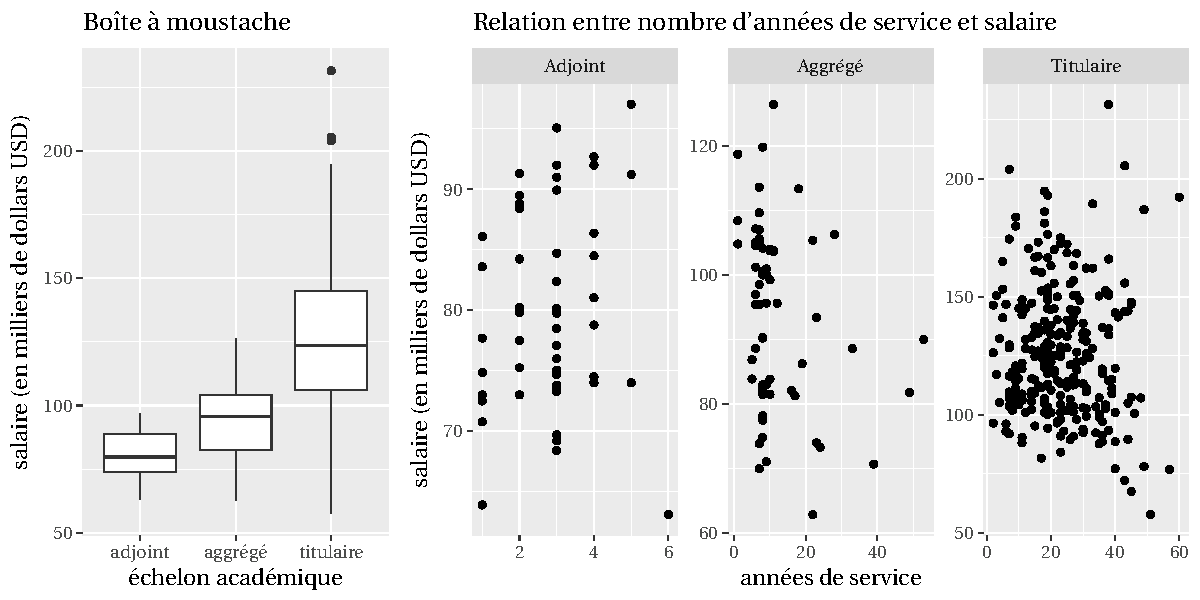
\includegraphics[width = 0.95\linewidth]{img/c5/06-correlated-salary_EDA_fr}  
 \end{center}
L'analyse exploratoire montre clairement que la variance au sein des échelons diffère.
\end{frame}

\begin{frame}[fragile]
\frametitle{Modéliser l'hétéroscédasticité de groupe}
\begin{tcolorbox}[colback=white, colframe=hecblue, title=Code \SASlang{} pour spécifier une variance différente pour chaque groupe]
\begin{small}
\begin{verbatim}
proc mixed data=modstat.college plots=studentpanel;
class sexe domaine echelon;
model salaire = sexe domaine echelon;
repeated / group = echelon;
run;
\end{verbatim}
\end{small}
\end{tcolorbox}
L'argument \texttt{repeated / group} renseigne \SASlang{} sur la structure des groupes.
\end{frame}
\begin{frame}
\frametitle{Estimés des variances des groupes et test de significativité}
 \begin{center}
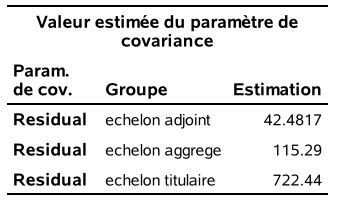
\includegraphics[width = 0.45\linewidth]{img/c5/diapos6-e25}  
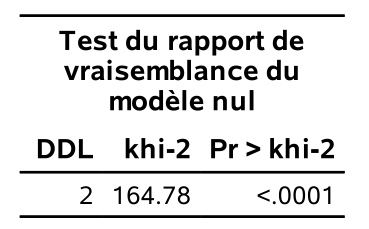
\includegraphics[width = 0.38\linewidth]{img/c5/diapos6-e26}  
 \end{center}
La variance croît avec l'échelon. Le test du rapport de vraisemblance montre que le modèle qui suppose des variances différentes au sein de chaque échelon est significativement meilleur que le modèle linéaire ordinaire, qui suppose une variance constante pour toutes les observations.
\end{frame}
\begin{frame}{Diagnostics graphiques pour les données \texttt{salaireprofs}}
  \begin{center}
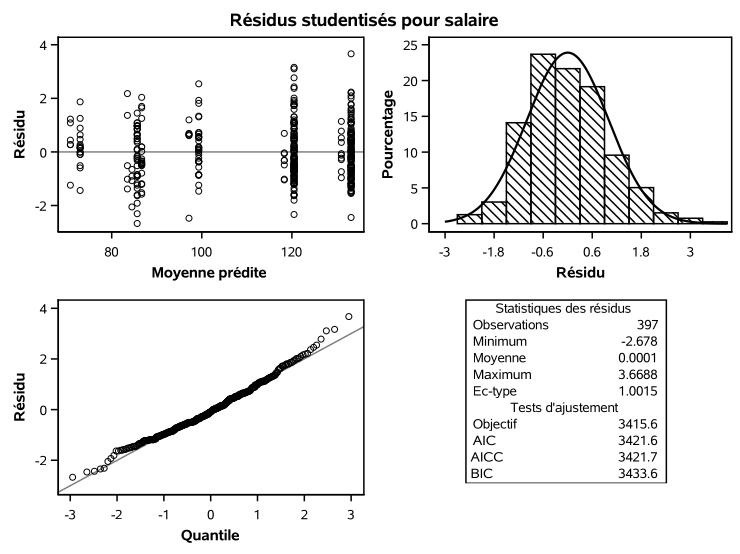
\includegraphics[width = 0.7\linewidth]{img/c5/diapos6-e28}  
 \end{center}
 Le diagramme des résidus studentisés versus les valeurs ajustées est conforme aux attentes. On peut être confiant pour notre inférence sur les paramètres de la moyenne.
\end{frame}
\begin{frame}
 \frametitle{Estimés des paramètres de la moyenne}
 \begin{center}
  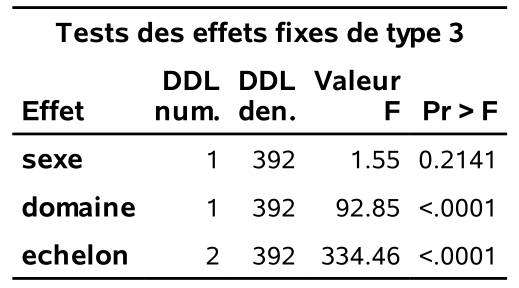
\includegraphics[width = 0.45\linewidth]{img/c5/diapos6-e27}  
 \end{center}

 \bi \item 
 Comparer le salaire des hommes et des femmes à l'aide d'un test-$t$ est incorrect, car le rang à un impact important sur le salaire.
 \item  Cela est dû à la plus faible proportion de femmes qui sont titulaires (7\%) que pour les adjointes et les aggrégées (16\%).
 \item Une fois que l'on a pris en compte l'hétéroscédasticité de groupe et l'effet de l'échelon, il n'y a pas de preuve de discrimination salariale et les écarts observés sont explicables.
 \ei
\end{frame}



\end{document}
